\documentclass{article} 

%\usepackage{amsmath,amsthm,amsfonts}
\usepackage[english]{babel}
\usepackage[numbers]{natbib}
\usepackage{rotating}
\usepackage{amsfonts,amsmath}
\usepackage{graphicx}
\usepackage{color} 
\usepackage[notref,notcite]{showkeys}
\usepackage{multirow}
\usepackage[utf8]{inputenc}
\usepackage[T2A]{fontenc}

\newcommand{\be}{\begin{equation}}
\newcommand{\ee}{\end{equation}}
\newcommand{\rf}[1]{(\ref{#1})}
\newcommand{\RR}{\mathbb{R}}
\newtheorem{thm}{Theorem}
\newtheorem{lm}{Lemma}

\begin{document}
\section{Увод}
Парадигматично уравнение на Бузинеск
\be\label{problemCh}
...
\ee
\section{Смяна на променливите}

За удобство правим следната смяна на променливите (виж \cite{ref25}):

\begin{align}
x = \sqrt{\beta_1} \bar{x}, \quad y = \sqrt{\beta_1} \bar{y}, \quad t = \sqrt{\beta_1} \bar{t} \nonumber
\end{align}
която променя основното уравнение \rf{problemCh} в
\be\label{problemVC}
 \beta (I-\Delta) \frac{\partial^2}{\partial t^2}u= 
(I-\Delta)\Delta u +\Delta( (\beta - 1 )u - \alpha \beta u^2 )
\ee
където $\beta = \beta_1/\beta_2$. 

Неограниченият домейн на уравнението е заменен с достатъчно голяма дискретна област $\Omega$, така че стойностите на неизвестната функция $u$ са достатъчно малки близо до границата $\partial \Omega$. Използвана е равномерна мрежа  $\Omega_h$ дефинирана по следния начин:

$$
\Omega_h = \{(x_i,y_j): x_i = (i-\frac{N_x-1}{2})h, y_j = (j-\frac{N_y-1}{2})h, i = 0,\cdots, N_x, j = 0 ,\cdots , N_y \},
$$

където $N_x$ и $N_y$ описват броя на точките по осите $x$ и $y$, а стъпката по пространството $h$ удовлетворява $h =2 L_x/(N_x-1) =2 L_y/(N_y-1)$.
С $2 L_x$ и $2 L_y$ са означени размерите на $\Omega_h$ по осите $x$ и $y$. Дискретния времеви интервал е дефиниран аналогично чрез
$$
T_{\tau} = \{(t_k): t_k = k\tau, k = 0,\cdots ,N_t \},
$$
където с $\tau = T/N_t$ сме означили стъпката по времето. Стойността на неизвестната функция $u$ в точка от мрежата $(x_i,y_j,t_k)$ е означена с $u_{i,j}^k$,т.е. долния индекс се използва за пространствената дискретизация, а горния за времева дискретизация.

\section{Запазване на дискретната енергия}
Нека да дефинираме оператора $A$, така че да удовлетворява $Av=-\Delta_h v=-v_{\bar{x}x} - v_{\bar{y}y}$. А сега да разгледаме диференчната схема

\be\label{FDS1}
\beta (E+A)v_{\bar{t}t}^k +\beta Av^k+A^2 v^k -\alpha \beta A\left(\frac{(v^{k+1})^3-(v^{k-1})^3}{3(v^{k+1}-v^{k-1})} \right)=0
\ee
Умножаваме \rf{FDS1} с $A^{-1}$ и получаваме
\be\label{FDS2}
\beta (E+A^{-1})v_{\bar{t}t}^k +\beta v^k+A v^k -\alpha \beta \frac{(v^{k+1})^3-(v^{k-1})^3}{3(v^{k+1}-v^{k-1})} = 0
\ee
Ако заместим $v^{k}=0.5(v^{k+1}+v^{k-1})-\frac{\tau^2}{2}v_{\bar{t}t}^k$ в \rf{FDS2} получаваме
\begin{align*}
&\left( \beta (E+A^{-1})- \frac{\tau^2}{2}(\beta E+A ) \right)v_{\bar{t}t}^k  + \frac{1}{2} (\beta E +A )(v^{k+1}+v^{k-1}) \\
&~~~~~-\alpha \beta \frac{(v^{k+1})^3-(v^{k-1})^3}{3(v^{k+1}-v^{k-1})} =0
\end{align*}
Умножаваме последното уравнение с $(v^{k+1}-v^{k-1})=\tau (v_{\bar{t}}^k + v_{t}^k)$, което важи за всяка точка от пространствената мрежа $(x_i,y_j) \in \Omega_h$, и сумираме получените уравнения в спрямо всички точки от мрежата. Така, след допълнителна реорганизация на членовете в уравнението получаваме, че
\be \label{num_en}
E_h(v^k) =E_h(v^{k-1}),
\ee
където
\begin{align*}
E_h(v^k)=\left( \left( \beta (E+A^{-1})- \frac{\tau^2}{4}(\beta E+A ) \right)v_{t}^k ,v_{t}^k \right)+\frac{1}{4} \beta \left(  v^{k+1}+v^{k}, v^{k+1}+v^{k} \right) \\
+\frac{1}{4}  \left(  A(v^{k+1}+v^{k}), v^{k+1}+v^{k} \right)
-\alpha \beta \frac{((v^{k+1})^3,1)+((v^{k})^3,1)}{3}.
\end{align*}
Така доказваме следната теорема
\begin{thm}
Решението получено от диференчната схема \rf{FDS1} запазва дискретната енергия $E_h(v^0)$, т.е.  $E_h(v^k) =E_h(v^{0})$ за всяко $k=1,2,...N_t$.
\end{thm}

\begin{thm}
Линейната диференчна схема съответстваща на \rf{FDS1} е условно устойчива, когато е изпълнено
$\tau^2 < \frac{\beta}{2}(1-\frac{\tau^2}{4}) h^2$.

\end{thm}
Доказателството е следствие от изследване на устойчивост при диференчни схеми в книгата на 
Самарский \cite{samarski}.

\section{Квадратурни формули за дискретните маса и енергия}

Масата при непрекъснатата задача \rf{problemVC} се дефинира като
\begin{equation}\label{intM}
D(u(x,y,t))=\int_{\RR^2} u(x,y,t)dx dy
\end{equation}
а енергията 
\begin{align}\label{ex-en}
E(u(x,y,t)):=&\int_{\RR^2} u_t(x,y,t) \left((A^{-1}+E)u_t(x,y,t)\right) dxdy+
\beta \int_{\RR^2} u^2(x,y,t) dxdy \nonumber\\
+& \int_{\RR^2}u(x,y,t) \left(A u(x,y,t)\right) dxdy
-\frac{2 \alpha \beta}{3} \int_{\RR^2} u^3(x,y,t) dxdy,
\end{align}
където $Au=-\Delta u$, а $D(u(x,y,t)) = D(u(x,y,0))$ and $E(u(x,y,t)) = E(u(x,y,0))$ са непрекъснатите маса и енергия за задачата \rf{problemVC} (виж \cite{ref1}). Нека да заменим оператора $Au=-\Delta u$ с неговата дискретна версия $-\Delta_h u$ като използваме апроксимаций от различен ред - $O(|h|^2)$, $O(|h|^4)$, $O(|h|^6)$. Ако имаме дискретната производната $u_t$ изчислена с апроксимации също от втори, четвърти и шести ред - $O(\tau^2)$, $O(\tau^4)$, $O(\tau^6)$ - то тогава може да приложим квадратурни формули за численото пресмятане на енергията \rf{ex-en}.

Следният интеграл
\begin{equation}\label{int}
D(u(x,y))=\int_{a_1}^{b_1} \int_{a_2}^{b_2} u(x,y)dx dy
\end{equation}

$x_i, ~i=0,1,...,N_x$; $x_0=a_1,~x_{N_x}=b_1$, $h_1=(b_1-a_1)/(N_x-1)$, 


$y_j, ~j=0,1,...,N_y$; $y_0=a_2,~y_{N_y}=b_2$,  $h_2=(b_2-a_2)/(N_y-1)$

може да се изчисли посредством двумерни квадратурни формули както е описано по-долу.

\subsection{ 2Д формула на трапците с глобална грешка $O(|h_1|^2+|h_2|^2)$ }

Апроксимацията на интеграла \eqref{intM} с глобална грешка $O(|h_1|^2+|h_2|^2)$ е

\begin{align}\label{quadr2}
D_h(u_{i,j}) =& \sum_{i=1}^{N_x-1} \sum_{j=1}^{N_y-1} h_1 h_2 u_{i,j}
+\frac{h_1}{2}\sum_{i=0} \sum_{j=1}^{N_y-1} h_2 u_{i,j}
+\frac{h_1}{2}\sum_{i=N_x} \sum_{j=1}^{N_y-1} h_2 u_{i,j} \nonumber\\
+&\frac{h_2}{2}\sum_{j=0} \sum_{i=1}^{N_x-1} h_1 u_{i,j}
+\frac{h_2}{2}\sum_{j=N_y} \sum_{i=1}^{N_x-1} h_1 u_{i,j}
\nonumber\\
+&\frac{1}{4}h_1 h_2 \left(u_{0,0}+u_{N_x,0}+u_{N_x,N_y}+u_{0,N_y}
\right).
\end{align}

\subsection{ 2Д правило на Симпсън с глобална грешка $O(|h_1|^4+|h_2|^4)$ error}

Нека да приемем, че $N_x=2k$, $N_y=2 l$. Така, за всяко $m=0,1,2,\cdots N_y$ пресмятаме, че

$$D_m= \frac{h_1 }{3} 
\left\{ u_{0,m}+u_{N_x,m}+ 4 \sum_{i=1}^{\frac{N_x}{2}}   u_{2i-1,m}
 +2 \sum_{i=1}^{\frac{N_x}{2}-1} u_{2i,m} \right\}.$$


От последната формула получаваме

\begin{equation}\label{quadr4}
D_h(u_{i,j}) =\frac{h_2 }{3} 
\left\{ D_{0}+D_{N_y}+ 4 \sum_{j=1}^{\frac{N_y}{2}}   D_{2j-1}
 +2 \sum_{j=1}^{{\frac{N_y}{2}}-1} D_{2j} \right\}
\end{equation}
апроксимацията на интеграла \eqref{intM} с глобална грешка $O(|h_1|^4+|h_2|^4)$.


\subsection{ 2D правило на Буул с глобална грешка $O(|h_1|^6+|h_2|^6)$}

Нека да приемем, че $N_x=4k$, $N_y=4 l$. Така, за всяко $m=0,1,2,\cdots N_y$ пресмятаме, че

\begin{align*}
D_m =& \frac{2h_1}{45} 
\left\{
7u_{0,m}+7u_{N_x,m}+32 \sum_{i=1}^{\frac{N_x}{2}}u_{2i-1,m}
+12\sum_{i=1}^{\frac{N_x}{4}}u_{4i-2,m}
+14 \sum_{i=1}^{\frac{N_x}{4}-1}u_{4i,m}
\right\}.
\end{align*}

Тогава формула \eqref{quadr6-2D} е апроксимацията на интеграла \eqref{intM} с глобална грешка $O(|h_1|^6+|h_2|^6)$.

\begin{align}\label{quadr6-2D}
&D_h(u_{i,j})  =
\frac{2h_2}{45} 
\left\{
7D_{0}+7D_{N_y}+32 \sum_{j=1}^{\frac{N_y}{2}}D_{2j-1}
+12\sum_{j=1}^{\frac{N_y}{4}}D_{4j-2}
+14 \sum_{j=1}^{\frac{N_y}{4}-1}D_{4j}
\right\}.
\end{align}

\section{Числени методи}

За всеки от разработените методи са изчислени масата и енергията върху полученото решение. То, заедно с неговите свойства като маса, енергия и форма са сравнени. Изчисленията са направени върху три вложени мрежи, за да се изследва сходимостта на методите. Показано е, че решенията получени с метода на Тейлор и Консервативната схема са доста близки. Една от целите на статията е да покаже, че метода на Тейлор приложен към уравнението \rf{problemVC} също води до достатъчно добри резултати, а също така може да се приложи с по-висок ред на апроксимация, което води и до по-фино решение.

\subsection{ Консервативна схема с крайни разлики }

Консервативната схема използва крайни разлики с втори ред на апроксимация, затова се предполага, че третите производни на непрекъснатото решение по времето и пространстово съществуват.  Тези апроксимациите са дефинирани както следва:

\be\label{difft}
\frac{\partial^2 u}{\partial t^2}(x_i, y_j, t_k ) = \frac{ u^{(k+1)}_{i, j} - 2u^{(k)}_{i,j} + u^{(k-1)}_{i,j} }{\tau^2} + O(\tau^2) 
\ee

\be\label{diffD}
\Delta u(x_i, y_j, t_k )  = \frac{ u^{(k)}_{i+1, j} - 2u^{(k)}_{i,j} + u^{(k)}_{i-1,j} }{h_1^2} + \frac{ u^{(k)}_{i, j+1} - 2u^{(k)}_{i,j} + u^{(k)}_{i,j-1} }{h_2^2} + O(h_1^2 + h_2^2) 
\ee
Като заместим дискретните диференциални оператори \rf{difft} и \rf{diffD} в \rf{problemVC} получаваме следното диференчно уравнение
\be\label{consFDS}
\beta (I-\Delta_h)\frac{ u^{(k+1)}_{i, j} - 2u^{(k)}_{i,j} + u^{(k-1)}_{i,j} }{\tau^2} = (\Delta_h - \Delta_h^2)u^{(k)}_{i,j} + \Delta_h(g(u^{(k)}_{i,j})),
\ee
%
където нелинейният член $g$ е дефиниран както следва:
\begin{align}
g(u^{(k)}_{i,j})=& -\frac{\alpha \beta} { 3 } \left( (u^{(k+1)}_{i,j})^2 + (u^{(k-1)}_{i,j})(u^{(k+1)}_{i,j}) + (u^{(k-1)}_{i,j})^2 \right) + \nonumber\\
+&\frac{ (\beta - 1 )}{ 2 }\left( u^{(k+1)}_{i,j} + u^{(k-1)}_{i,j} \right).
\end{align}

Това не е тривиална апроксимация на $g$, а такава с която дискретната енергия се запазва, т.е. е константна функция по отношение на времевата променлива $t$ (виж \cite{ref20}). Да отбележим, че Консервативната схема \rf{consFDS} е имплицитна тъй като нелинейният член зависи от горния слой по времето. Така на всеки слой по времето се правят итераций на Пикард, за да разрешим неизвестната дискретна функция $u^{(k+1)}_{i,j}$.

\subsection{ Метод на Тейлор }

Методът на Тейлор използва развитие в ред спрямо времевата променлива на търсената функция $u(x,y,t)$. Но за извеждането на крайните разлики за пресмятане на производните по пространството също се използва развитие в ред на Тейлор. Затова се предполага, че решението е $p+1$ кратна гладка функция спрямо всички аргументи $x$, $y$ and $t$, т.е. $u \in C^{p+1,p+1,p+1}(\Omega \times T)$ като при следващите изчисления описани по долу са използвани стойностите $p=2,4,6$.
За дискретизацията на оператора на Лаплас са използвани централни крайни разлики с различна степен на апроксимация:
\begin{equation}\label{fd}
u_{\widehat{xx},p}(x,y) :=  \frac{1}{h^2} \sum\limits_{i=-p/2}^{p/2} d_i u(x+ih, y_j).
\end{equation}
като теглата $d_i$ са взети от \cite{forn} и са описани в Таблица \ref{table:A00}. Производните по $y$ са дефинирани аналогично със същия шаблон.
\begin{table}[ht]
\centering
\small
		\begin{tabular}{||c|l|l|l|l|l|l|l||}
			\hline
			\hline
            $p=2$          &          &                                 &     1      &   -2   &    1    &    &        \\
   			\hline 
			\hline 
           $p=4$          &                            &   $-\frac{1}{12}$     &     $\frac{4}{3}$      &   $-\frac{5}{2} $     &    $\frac{4}{3}$    &  $-\frac{1}{12}$   &        \\
	   \hline
			\hline 
            $p=6$        &   $\frac{1}{90}$       &     $-\frac{3}{20}$     &    $\frac{3}{2}$      &    $-\frac{49}{18}$   &    $\frac{3}{2}$    & $-\frac{3}{20}$    &    $\frac{1}{90}$       \\
	   \hline
			\hline 
		\end{tabular}
	\caption{ Finite differences used for the approximation of the Laplace operator.}
	\label{table:A00}
\end{table}

Грешката от апроксимациите \rf{fd} са $O(h^p)$ в зависимост от избора на $p$. Нека да означим с $u_{i,j}(t)$ апроксимацията на неизвестната функция $u$ в точка от мрежата $(x_i, y_j)$ за произволно време $t$. Непрекъснатият оператор на Лаплас в уравнение \rf{problemVC} се заменя с дискретния $\Delta_{h,p} = u_{\widehat{xx},p} + u_{\widehat{yy},p}$, което води до следната система от ОДУ:
\be \label{DiscreteEq}
\beta (I-\Delta_{h,p}) \frac{\partial^2 u}{\partial t^2}(x_i, y_j, t)=
 (I - \Delta_{h,p})\Delta_{h,p} u_{i, j}(t) + \Delta_{h,p} ( g( u_{i, j}(t) ) )
\ee
за всяка точка от мрежата $(x_i, y_j)$, където $i = 0..N_x$, $j=0..N_y$. За всяко едно ОДУ от системата се прави развитие в ред на Тейлор спрямо времевата променлива:
\begin{align} \label{TSe}
u(x_i, y_j, t+\tau) = u(x_i, y_j, t) + \tau \frac{ \partial u }{ \partial t }(x_i, y_j, t)  + ... 
%\nonumber
%\\
\frac{ \tau^p }{ p! } \frac{ \partial^p u }{ \partial t^p }(x_i, y_j, t) + O(\tau^{p+1})
\end{align}
при $p \ge 2$. Редът на апроксимация по времето зависи от броя на членовете $p+1$, които участват в реда на Тейлор. По този начин реда на апроксимация по времето и пространството е еднакъв и зависи от избора на $p$, което по-късно спомага за тестването на сходимостта. Всяка точка от мрежата представлява начало на крива, чиято траектория се описва с развитието на Тейлор \rf{TSe}. Изчисляването на формула \rf{TSe} е рекурсивен процес като всеки член от сумата се пресмята отделно. Например, при $t=0$ първите два члена са известни от началното условие ($u_0$, $u_1$), а третият се получава чрез дискретното уравнение \rf{DiscreteEq}. За намиране на последното се използват Fast Poisson Solvers за обръщане на оператора $I-\Delta_{h,p}$ представен от дясната страна на уравнението. Чрез диференциране на уравнение \rf{DiscreteEq} по времето се получават зависимости за по-високи производни $\frac{\partial^3 u}{\partial t^3}$, $\frac{\partial^4 u}{\partial t^4}$, $\frac{\partial^5 u}{\partial t^5}$ и т.н.  Това е итеративен процес, където например петата производна зависи от третата, втората, първата и нулевата, третата зависи от първата и нулевата. След като всички необходими производни са пресметнати се заместват в уравнение \rf{TSe} и така се получават следните апроксимации: за $p=2$ имаме $O(|h|^2 + \tau^2)$, за $p=4$ - $O(|h|^4 + \tau^4)$ и за $p=6$ - $O(|h|^6 + \tau^6)$. Тук е важно да се отбележи, че е необходимо да се пресметне и развитието в ред на Тейлор за първата производна по времето $u_t(x_i, y_j, t+\tau)$, която е сходна с \rf{TSe} и има същия ред на апроксимация. Това е необходимо тъй като решението на следващия слой по времето зависи от двойката ($u$, $u_t$), която служи като базис и всички по-високи производни могат да се изразят единствено чрез нея.

Сложността на алгоритъма зависи от големината на областа в която се разглежда числената задача,
$$ O( N_x N_y N_t ) $$
където $N_x N_y$ е броя на точките в $\Omega_h$ и $N_t = T/\tau$. Повечето от изчислителното време се отделя за обръщане на оператора $I-\Delta_{h,p}$ в уравнение \rf{DiscreteEq}, което е необходимо за $N_x N_t$ обръщания на $p+1$ лентова матрица с размери ($N_y \times N_y$). Избора на $p$, който е направен тук увеличава сложността с константа, което води до линейна зависимост на времето за изчисление спрямо броя на точките в областта. 

\section{Числени резултати}

Първоначално е представен редът на сходимост при Консервативната схема за дискретните решение и енергия. Впоследствие, същото е направено и за метода на Тейлор. При валидацията на масата са направени допълнителни изчисления, за да се обясни нейното поведение. Най-накрая са сравнени решенията между двата различни подхода. Дискретните енергия и маса се пресмятат на всяка стъпка по времето и са вектори с дължина $N_t$. При Консервативната схема, енергията се пресмята с правилото на трапците, а при метода на Тейлор с правилата на трапците, Симпсън и Буул съответно с грешка от апроксимациите $O(h^{2} + \tau^2 )$, $O(h^{4} + \tau^4 )$ и $O(h^{6} + \tau^6 )$. Сходимостта на изследваните крайни разлики и развития в ред на Тейлор е получена послредством правилото на Рунге:
\begin{equation}\label{Runge}
\xi = ln  \frac{\Vert u_{h,\tau} - u_{(h,\tau)/2} \Vert_\kappa } {\Vert  u_{(h,\tau)/2} - u_{(h,\tau)/4} \Vert_\kappa  } | / ln(2),
\end{equation}
когато не е известно аналитично решение на уравнението. Формула \rf{Runge} е използванa и при изчислението на сходимостта на дискретната енергията върху три вложени мрежи с размери $[0:\tau:T]$, $[0:\tau/2:T]$ and $[0:\tau/4:T]$. Числените резултати са извършени при следните два случая (виж Таблица \rf{tableP}) $\beta = 3$, $c=0.45$ и $\beta = 1$, $c=0.9$ \begin{table}
\centering
\small
		\begin{tabular}{||c|l|l|l|l|l|l|l||}
			\hline
			\hline
                                            &    $\beta$, $c$                              & $O(|h|^p+\tau^p)$   &      $h$                                & $L_x$,$L_y$                              &  Методи & $T$      & Гр. Усл.  \\
   			\hline 
					\hline
           Test 1                        &      $\beta = 3$     &      $p=2, 4, 6$    &    $h=0.2,$       & $L_x = 30$                & Тейлор &                10    &    нула  \\
                                             &      $c=0.45$         &                             &    $ 0.1, 0.05$   & $L_y=27$                  &  Конс. сх. &                &            \\
	   \hline
			\hline 
           Test 2                        &      $\beta = 1$     &      $p=2, 4, 6$    &     $h=0.4,$       & $L_x = 128$         & Тейлор  &               10    &   нула  \\
                                             &      $c=0.9$           &                             &      $0.2, 0.1$     & $L_y=58$              & Конс. сх.  &                   &     \\
	   \hline
			\hline 
		\end{tabular}
\caption{Параметрична таблица с описание на числените тестове}
\label{tableP}
\end{table}
с последващите уточнения. Първо, Консервативната схема е приложена само с втори ред на апроксимация  $p=2$. Второ, при $p=2$ дискретната стъпка по времето е 
 $\tau=h/200$, иначе при $p=4, 6$ тя е $\tau = h/10$. Трето, всички изчисления използват нулево гранично условие, т.е. стойностите на нейзвестната функция в шаблона от крайните разлики, които се намират извън числената област $[-L_x, L_x] \times [-L_y, L_y]$ са нули.

\subsection{Ред на сходимост при Консервативната схема}

Таблица \ref{tableC} показва скоростта на сходимост на численото решение по правилото на Рунге \rf{Runge} върху три вложени мрежи. При Консервативната схема са приложени крайни разлики само от втори порядък на апроксимация, т.е. $p=2$ при Тест 1 и Тест 2 представени в първата колона от таблицата. Стъпките по времето и пространството са описани във втората колона. В следващите две колони са представени апроксимационните грешки  $\Vert u_{h,\tau} - u_{(h,\tau)/2} \Vert_\kappa$, $\Vert  u_{(h,\tau)/2} - u_{(h,\tau)/4} \Vert_\kappa$ в $L_2$ и $L_{\infty}$ норми както и скоростта на сходимост.

%C
\begin{table}[ht]
\centering
\small
		\begin{tabular}{||c|l|ll|ll||}
			\hline
			\hline
      \multirow{2  }{*}{FDS}        & \multirow{2  }{*}{$h$, $\tau$}  & Ап. грешки      &Ред на& Ап. грешки        &Ред на   \\
	                                        &                                                     &  $E_i$в$L_2$ &  сход. & $E_i$в$L_\infty$  & сход. \\
   			\hline 
					\hline 
  $\beta=3$                &0.2, 0.001         &                    &                &                  &                   \\
   c=0.45                     &0.1, 0.0005         & 0.989422   &                & 1.043649  &                   \\
     $O(h^2 + \tau^ 2)$ &0.05, 0.00025  &0.344818    & 1.52       & 0.355517   &   1.55   \\
	   \hline
			\hline 
       $\beta=1$           & 0.4, 0.002       &                   &           &                 &   \\
                  c=0.9       & 0.2, 0.001        & 0.200424   &          &0.072726  &   \\
  $O(h^2+ \tau^2)$  & 0.1, 0.0005       & 0.047899   & 2.06  &0.021451  & 1.76 \\
	   \hline
			\hline 
		\end{tabular}
		\caption{Скорост на сходимост на численото решение при Консервативната схема с нулево гранично условие и грешки от апроксимацията $O(h^{2} + \tau^2 )$. Грешките $E_i$ са измерени в $L_2$ и $L_\infty$ норми}
\label{tableC}
\end{table}

%D
\begin{table}[ht]
\centering
\small
		\begin{tabular}{||c|l|ll|ll||}
			\hline
			\hline
      \multirow{2  }{*}{FDS}        & \multirow{2  }{*}{$h$, $\tau$}  & Ап. грешки      &Ред на& Ап. грешки        &Ред на   \\
	                                        &                                                     &  $E_i$в$L_2$ &  сход. & $E_i$в$L_\infty$  & сход. \\
   			\hline 
					\hline 
  $\beta=3$                &0.2, 0.005         &                    &                &                  &                   \\
   c=0.45                     &0.1, 0.0025         & 0.044442   &                & 0.444423  &                   \\
     $O(h^2 + \tau^ 2)$ &0.05, 0.00025  & 0.007831   & 2.50       & 0.110750  & 2.00   \\
	   \hline
			\hline 
       $\beta=1$           & 0.4, 0.002       &                   &           &                 &   \\
                  c=0.9       & 0.2, 0.001        & 0.051409   &          &0.363515  &   \\
  $O(h^2+ \tau^2)$  & 0.1, 0.0005       & 0.008939   & 2.52  &0.089393  & 2.02  \\
	   \hline
			\hline 
		\end{tabular}
		\caption{Скорост на сходимост на дискретната Енергия при Консервативната схема с нулево гранично условие и грешки от апроксимацията $O(h^{2} + \tau^2 )$. Грешките $E_i$ са измерени в $L_2$ и $L_\infty$ норми}
\label{tableD}
\end{table}

Таблица \ref{tableD} е аналогична с Таблица \ref{tableC}, но показва скоростта на сходимостта на дискретната Енергия \rf{ex-en}. Вижда се, че резултатите от двете таблици са близки и съизмерими с използвания втори ред на апроксимация.

\subsection{Ред на сходимост при метода на Тейлор (метод на Линиите)}

В таблица \ref{tableA} е представен редът на сходимост от численото решение. При методът на Тейлор са използвани апроксимации от втори, четвърти и шести ред, т.е. $p=2,4,6$ за Тест 1 и Тест 2 от първата колона в таблицата. Тук отново са направени изчисления върху три вложени мрежи с различни стъпки по времето и пространстово, които са показани във втората колона. В следващите две колони са представени апроксимационните грешки  $\Vert u_{h,\tau} - u_{(h,\tau)/2} \Vert_\kappa$, $\Vert  u_{(h,\tau)/2} - u_{(h,\tau)/4} \Vert_\kappa$ в $L_2$ и $L_{\infty}$ норми както и редът на сходимост. Стойностите на сходимост отговарят на приложения ред на апроксимация. Само при Тест 2, $O(h^6 + \tau^6)$ и $L_2$ норма, сходимостта $4.86$ е малко по-ниска от очакваното. Този резултат се отдава на нулевото гранично условие заедно с използвания седем точков шаблон по границата при апроксимация $O(h^6 + \tau^6)$.
%A
\begin{table}[ht]
\centering
\small
		\begin{tabular}{||c|l|ll|ll||}
			\hline
			\hline
      \multirow{2  }{*}{FDS}        & \multirow{2  }{*}{$h$, $\tau$}  & \multirow{2  }{*}{errors $E_i$in$L_2$}  &Conv.& \multirow{2  }{*}{errors $E_i$in$L_\infty$}  &Conv.  \\
	         &                    &                               & Rate   &                                        & Rate \\
   			\hline 
					\hline 
  $\beta=3$                &0.2, 0.001          &              &              &                     &      \\
   c=0.45                     &0.1, 0.0005          &0.989414 &            &1.043641    &       \\
     $O(h^2 + \tau^ 2)$ &0.05, 0.00025   & 0.344813 & 1.52    &0.355511    &  1.55      \\
			\hline 
  $\beta=3$               &0.2, 0.02       &              &            &                     &      \\
   c=0.45                    &0.1, 0.01      &0.191224 &            &0.193874    &       \\
     $O(h^4+ \tau^4)$ &0.05, 0.005&0.013029 & 3.87   &0.013656     &3.82       \\
			\hline 
  $\beta=3$               &0.2, 0.02       &                &            &                     &      \\
     c=0.45                 &0.1, 0.01        &0.032671 &            &  0.033626    &       \\
     $O(h^6+ \tau^6)$ &0.05, 0.005 &0.000598 &5.77     & 0.000635    & 5.72       \\
	   \hline
			\hline 
       $\beta=1$       &0.4, 0.002        &             &            &           &   \\
                  c=0.9    &0.2, 0.001       &  0.20366   &            &0.075854 &   \\
  $O(h^2+ \tau^2)$ &0.1, 0.0005   &0.048320   &2.07  &0.022307  & 1.77 \\
			\hline
      $\beta=1$               &0.4, 0.04    &            &               &             &    \\
       c=0.9                     &0.2, 0.02     & 0.028275   &        &  0.013518   &   \\
       $O(h^4+ \tau^4)$ &0.1, 0.01   &0.001812 & 3.96  & 0.000971  & 3.80  \\
    \hline
  $\beta=1$     &0.4, 0.04   &            &          &                  &      \\
      c=0.9                    &0.2, 0.02   &0.006734 &           & 0.003338      &       \\
     $O(h^6+ \tau^6)$ &0.1, 0.01 & 0.000232 &4.86 & 0.000069  & 5.60        \\
	   \hline
			\hline 
		\end{tabular}
		\caption{Скорост на сходимост на численото решение при Консервативната схема с нулево гранично условие и грешки от апроксимацията $O(h^{2} + \tau^2 )$, $O(h^{4} + \tau^4 )$ and $O(h^{6} + \tau^6 )$. Грешките $E_i$ са измерени в $L_2$ и $L_\infty$ норми}
\label{tableA}
\end{table}

Table \ref{tableB} has analogous structure as Table \ref{tableA} and measures the convergence rate based on the results of the discrete Energy \rf{ex-en}. The convergence rate of the Energy corresponds to the approximation order that is used. Only for Test 2 and $O(h^6 + \tau^6)$ the convergence results $4.45$ and $4.68$ for $L_2$ and infinity norms are slightly less than expected. Analogously to the previous Table \ref{tableA} where the $L_2$ is out of expected order, this result could be due to the zero boundary conditions. The evaluation of the Energy functional \rf{ex-en} involves quadrature formulas which implies similar behavour to the $L_2$ norm. Thus, the infinity norm results in a similar convergence rate $4.68$ for the problematic case.
% When using zero boundary conditions all points on the finite difference stencil that are outside the numerical domain $\Omega_h$ are zeros. This creates a jagged solution surface on the boundary.
For the $O(h^2 + \tau^2)$ case ( both Test 1 and Test 2), much smaller time step  $\tau = h/200$ is used. This results in solutions which are similar in shape and form for the three nested meshes. If the step is chosen bigger (e.g. $\tau = h/10$), then the difference in the solution shape between $O(h^2 + \tau^2)$ and the other $O(h^4 + \tau^4)$ and $O(h^6 + \tau^6)$ approximations is much larger. 

%B
\begin{table}[ht]
\centering
\small
		\begin{tabular}{||c|l|ll|ll||}
			\hline
			\hline
      \multirow{2  }{*}{FDS}        & \multirow{2  }{*}{$h$, $\tau$}  & \multirow{ 2 }{*}{errors $E_i$in$L_2$}  &Conv.& \multirow{2  }{*}{errors $E_i$in$L_\infty$}  &Conv.  \\
	                                        &                                                     &                                                                 &  Rate &                                                                       & Rate \\
   			\hline 
					\hline 
  $\beta=3$                &0.2, 0.001         &              &            &                     &      \\
   c=0.45                     &0.1, 0.0005         &0.044442  &            &0.444425 &       \\
     $O(h^2 + \tau^ 2)$ &0.05, 0.00025  & 0.007831 & 2.50      & 0.110750     & 2.00      \\
			\hline 
  $\beta=3$               &0.2, 0.02       &                &            &                     &      \\
   c=0.45                    &0.1, 0.01      &0.018288 &            &0.072718   &       \\
     $O(h^4+ \tau^4)$ &0.05, 0.005  &0.000945 &4.27    &0.002997   &4.60      \\
			\hline 
  $\beta=3$               &0.2, 0.02       &                &            &                      &            \\
     c=0.45                 &0.1, 0.01        &0.027425 &            &  0.122934    &           \\
     $O(h^6+ \tau^6)$ &0.05, 0.005 &0.000318 & 6.42     & 0.001467     &6.38   \\
	   \hline
			\hline 
       $\beta=1$       &0.4, 0.002        &             &            &           &   \\
                  c=0.9    &0.2, 0.001       &  0.046343   &            &0.352955 &   \\
  $O(h^2+ \tau^2)$ &0.1, 0.0005   &0.007430   &2.64  &0.086470  & 2.02 \\
			\hline
      $\beta=1$               &0.4, 0.04    &            &               &             &    \\
       c=0.9                     &0.2, 0.02     & 0.023067   &        &  0.040550   &   \\
       $O(h^4+ \tau^4)$ &0.1, 0.01   &0.001411 & 4.03   & 0.003203  & 3.66  \\
    \hline
  $\beta=1$     &0.4, 0.04   &            &          &                  &      \\
      c=0.9                    &0.2, 0.02   &0.010898 &           & 0.032597      &       \\
     $O(h^6+ \tau^6)$ &0.1, 0.01 & 0.000496 &4.45 & 0.001266  & 4.68        \\
	   \hline
			\hline 
		\end{tabular}
		\caption{Convergence speed for the Energy using Taylor method with zero boundary conditions and different approximation errors $O(h^{2} + \tau^2 )$, $O(h^{4} + \tau^4 )$ and $O(h^{6} + \tau^6 )$. Errors $E_i$ are measured in $L_2$ and $L_\infty$ norms.}
\label{tableB}
\end{table}

\subsection{Numerical Results for the Mass and Energy}

Figure \ref{Test1En} shows the discrete Mass and Energy for Test 1 calculated using solutions from the Conservative FDS and Taylor method. Figure \ref{Test2En} shows analogous results for Test 2. In case of $O(|h|^2 +\tau^2)$ the Mass and Energy realized by both methods for Test 1 and Test 2 overlap (dark line and blue circles). The Energy graphs are constant functions over the time interval.
\begin{figure}[ht]\vspace{0.2cm}
	\begin{minipage}[b]{0.4\linewidth}
		 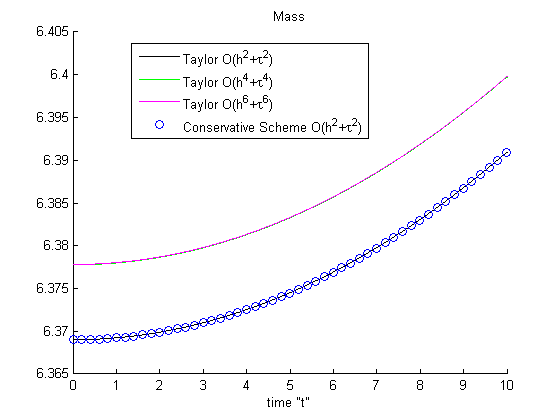
\includegraphics[width=\linewidth]{../amitans/figures/Mass_bt3_c045_h005_Taylor_Conservative.png}
	\end{minipage}	
	\begin{minipage}[b]{0.4\linewidth}
		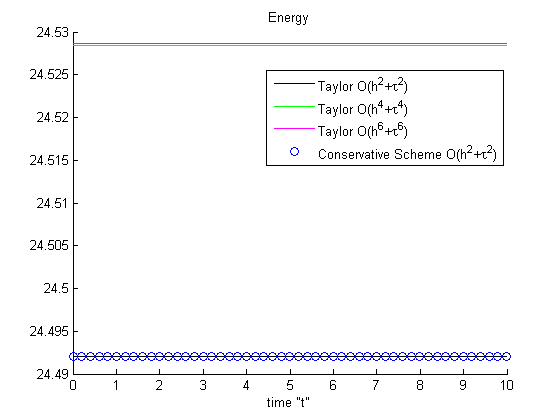
\includegraphics[width=\linewidth]{../amitans/figures/Energy_bt3_c045_h005_Taylor_Conservative.png}	
	\end{minipage}
\caption{The Mass (left) and Energy (right) of the solution for Test 1, $O(|h|^2 + \tau^2)$ and $T=10$.}
\label{Test1En}
\end{figure}

The Mass increases slightly over the time interval but the gain is neglectable compared to the initial value. For Test 1 the increase with respect to the initial Mass is $0.33\%$ and for Test 2 is $1.8\%$.

\begin{figure}[ht]\vspace{0.2cm}
	\begin{minipage}[b]{0.4\linewidth}
		 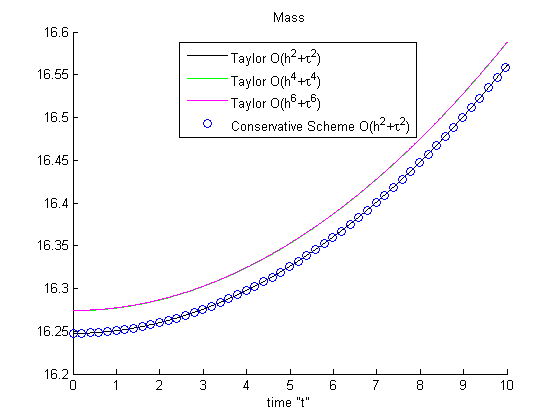
\includegraphics[width=\linewidth]{../amitans/figures/Mass_bt1_c090_h010_Taylor_Conservative.png}
	\end{minipage}	
	\begin{minipage}[b]{0.4\linewidth}
		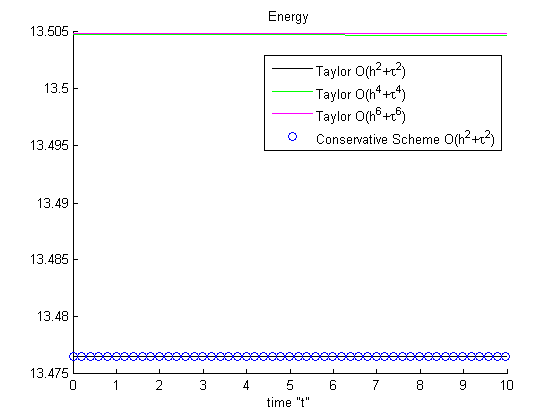
\includegraphics[width=\linewidth]{../amitans/figures/Energy_bt1_c090_h010_Taylor_Conservative.png}
		
	\end{minipage}
\caption{The Mass (left) and Energy (right) of the solution for Test 2, $O(|h|^2 + \tau^2)$ and $T=10$.}
\label{Test2En}
\end{figure}

For the Taylor Method, the discrete Mass and Energy in Figure \ref{Test1En} and \ref{Test2En} are calculated with three different approximations, namely, trapezoidal formula \rf{quadr2} with $O(h^2)$, Simpson's Rule \rf{quadr4} with $O(h^4)$ and Boole's Rule \rf{quadr6-2D} with $O(h^6)$. It is observed that increasing the order of approximation does not affect the gain for the Mass. It is also confirmed that decreasing the step size $h$ produces similar result, i.e. the graph is slightly shifted upwards or downwards. In the next computations, in order to validate the proper behaviour of the Mass, only the size of the domain is changed whereas the approximation order and discrete steps are fixed.
%----------------------------------------------------------------------------------------------------------------------------------------------
\iffalse
\begin{figure}[ht]\vspace{0.4cm}
	\begin{minipage}[b]{0.33\linewidth}
		 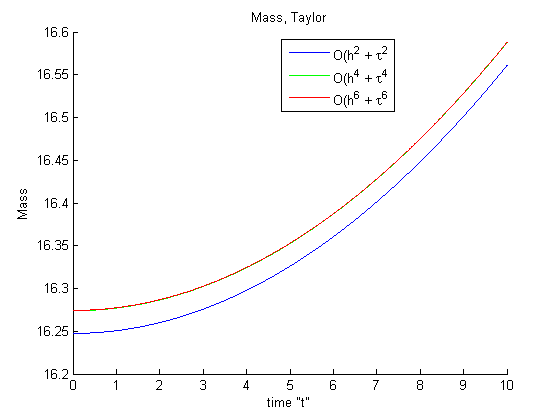
\includegraphics[width=\linewidth]{../amitans/figures/Mass_bt1_c090_h010_x3O.png}
	\end{minipage}	
	\begin{minipage}[b]{0.33\linewidth}
		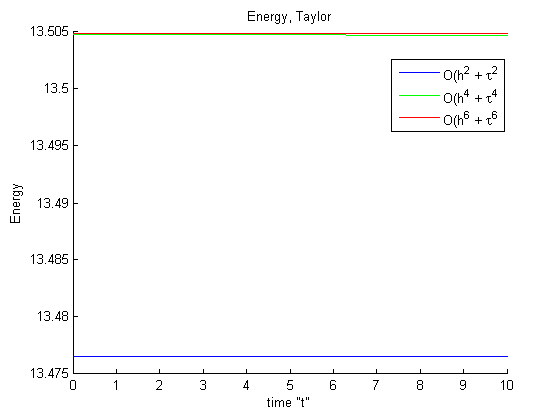
\includegraphics[width=\linewidth]{../amitans/figures/Energy_bt1_c090_h010_x3O.png}
		
	\end{minipage}
\caption{The Mass (left) and Energy (right) of the Taylor solution for Test 1, $O(|h|^2 + \tau^2)$, $O(|h|^4 + \tau^4)$, $O(|h|^6 + \tau^6)$ and $T=10$.}
\label{Test1TEn}
\end{figure}
\begin{figure}[ht]\vspace{0.4cm}
	\begin{minipage}[b]{0.33\linewidth}
		 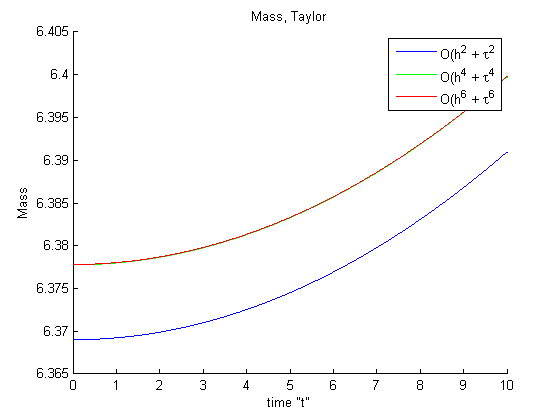
\includegraphics[width=\linewidth]{../amitans/figures/Mass_bt3_c045_h005_x3O.png}
	\end{minipage}	
	\begin{minipage}[b]{0.33\linewidth}
		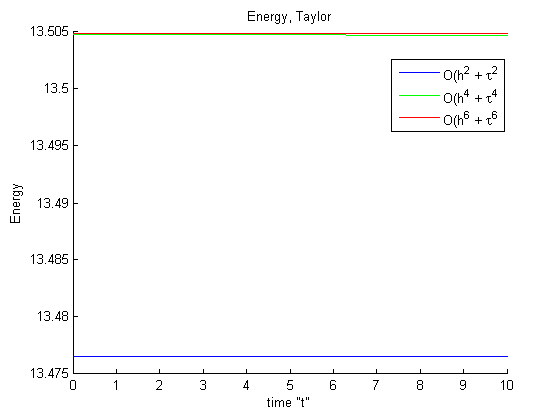
\includegraphics[width=\linewidth]{../amitans/figures/Energy_bt1_c090_h010_x3O.png}
		
	\end{minipage}
\caption{The Mass (left) and Energy (right) of the Taylor solution for Test 2, $O(|h|^2 + \tau^2)$, $O(|h|^4 + \tau^4)$, $O(|h|^6 + \tau^6)$ and $T=10$.}
\label{Test2TEn}
\end{figure}
\fi
%----------------------------------------------------------------------------------------------------------------------------------------------
If $D$ denotes the discrete Mass, then the percentage gain for the Mass is defined by $100 \times |D(t=0) - D(t=T)|/D(t=0)$. On Figure \ref{Test1_2Mass} one could see that by increasing the size of the domain $\Omega_h$ the gain for the Mass decreases. Taylor method with sixth approximation order and largest step sizes is applied to create the graphs. On the left panel three different domains of size $[-30, 30] \times [-27, 27]$, $[-60, 60] \times [-54, 54]$ and $[-120, 120] \times [-108, 108]$ are used. Furthermore, the used parameter set is $\beta =  3$, $c = 0.45$ (Test 1) and $h=0.2$. The percentage gain for the Mass when increasing the domain is $0.33\%$, $0.11\%$ and $0.06\%$. Analogously, on the right panel, the domains are $[-128, 128] \times [-58, 58]$, $[-256, 256] \times [-116, 116]$ and $[-512, 512] \times [-232, 232]$. The parameter set is $\beta =  1$, $c = 0.9$ (Test 2) and $h=0.4$. Here, the percentage gain for the Mass when increasing the domain is $1.80\%$, $0.70\%$ and $0.18\%$.
\begin{figure}[ht]\vspace{0.2cm}
	\begin{minipage}[b]{0.4\linewidth}
		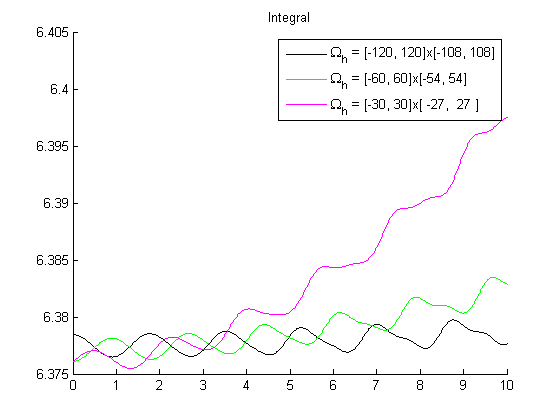
\includegraphics[width=\linewidth]{../amitans/figures/MassTaylor_120_60_30_ZB1_bt3_c045_h020_O(h^6).png}
	\end{minipage}	
	\begin{minipage}[b]{0.4\linewidth}
		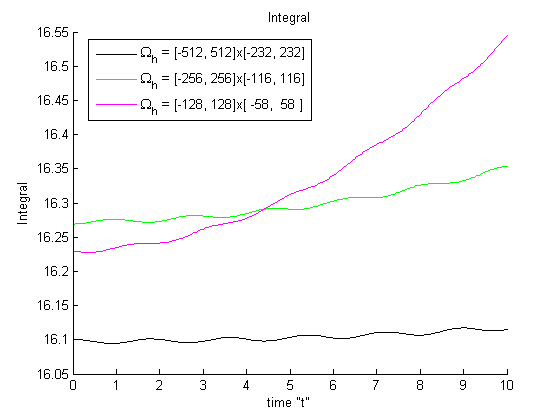
\includegraphics[width=\linewidth]{../amitans/figures/MassTaylor_512_256_128_ZB1_bt1_c090_h040_O(h^6).png}
		
	\end{minipage}
\caption{The Mass of the Taylor solution for approximation $O(|h|^6 + \tau^6)$ and $T=10$ over three nested domains. Left panel is for $\beta =  3$, $c = 0.45$ and right panel is for $\beta =  1$, $c = 0.9$.}
\label{Test1_2Mass}
\end{figure}

\subsection{Numerical Results for the shape and maximum of the solution}

The following paragraph discusses the shape of the solution obtained by the Conservative FDS and Taylor method. The set up for the calculations is described in Table \ref{tableP} when $p=2$, i.e. both Test 1 and Test 2 are done on three nested meshes. For each Test and mesh both solution techniques are applied with second approximation order. Let us denote with $uC$ and $uT$ the solutions obtained by the Conservative scheme \rf{consFDS} and the TS expansion \rf{TSe}. Figures \ref{Test1_Diff} and \ref{Test2_Diff} show the solution difference for Test 1 and Test 2 respectively. The pictures cover only the center of the domain $\Omega_h$ where the values of the difference are higher. This is one nineth of all mesh points.
\begin{figure}[ht]\vspace{0.4cm}
	\begin{minipage}[b]{0.32\linewidth}
		 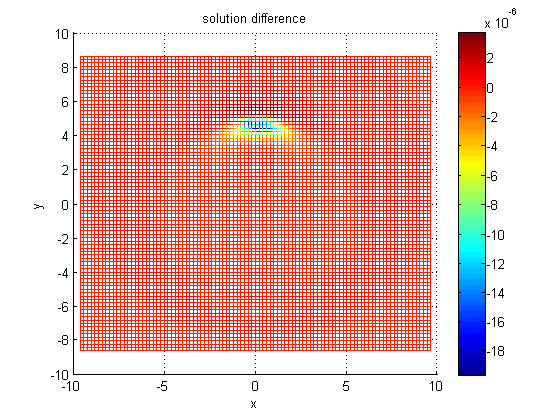
\includegraphics[width=\linewidth]{../amitans/figures/compare_30_bt3_c045_h020.png}
	\end{minipage}	
	\begin{minipage}[b]{0.32\linewidth}
		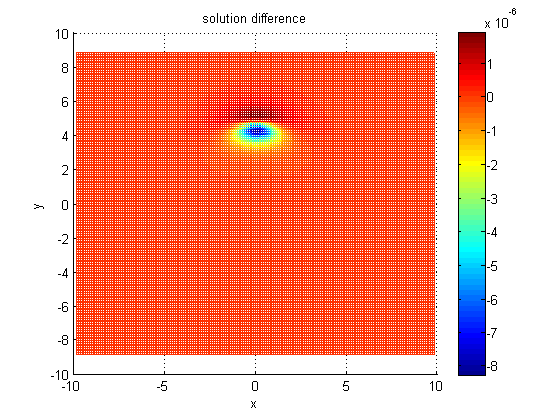
\includegraphics[width=\linewidth]{../amitans/figures/compare_30_bt3_c045_h010.png}
	\end{minipage}	
	\begin{minipage}[b]{0.32\linewidth}		
		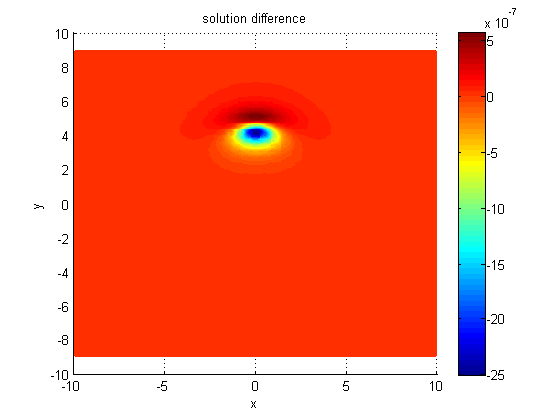
\includegraphics[width=\linewidth]{../amitans/figures/compare_30_bt3_c045_h005.png}
	\end{minipage}
\caption{Difference $uC - uT$ between solutions from Conservative Scheme and TS approach at time $t=10$, $O(|h|^2 + \tau^2)$ for Test 1. From Left to right $h=0.2, 0.1, 0.05$.}
\label{Test1_Diff}
\end{figure}

\begin{figure}[ht]\vspace{0.4cm}
	\begin{minipage}[b]{0.32\linewidth}
		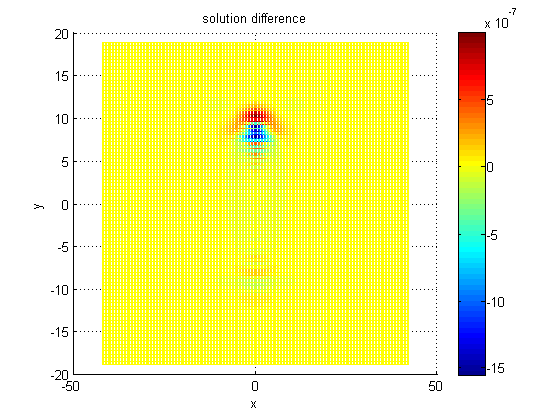
\includegraphics[width=\linewidth]{../amitans/figures/compare_128_bt1_c09_h040.png}
	\end{minipage}	
	\begin{minipage}[b]{0.32\linewidth}
		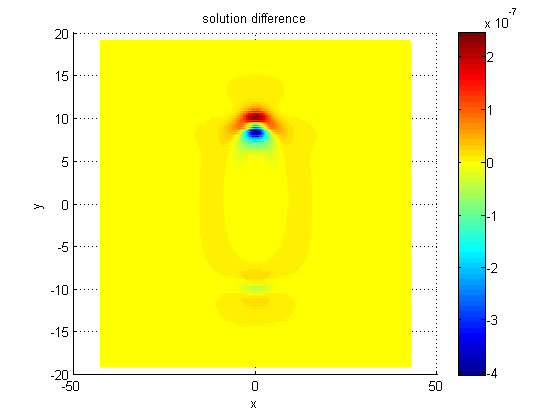
\includegraphics[width=\linewidth]{../amitans/figures/compare_128_bt1_c09_h020.png}
	\end{minipage}	
	\begin{minipage}[b]{0.32\linewidth}
		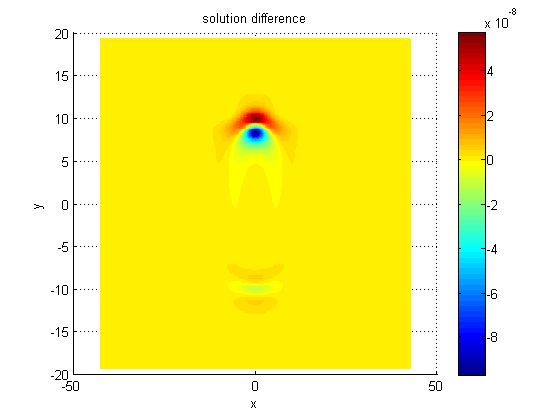
\includegraphics[width=\linewidth]{../amitans/figures/compare_128_bt1_c09_h010.png}
	\end{minipage}
\caption{Difference $uC - uT$ between solutions from Conservative Scheme and TS approach at time $t=10$, $O(|h|^2 + \tau^2)$ for Test 2. From Left to right $h=0.4, 0.2, 0.1$.}
\label{Test2_Diff}
\end{figure}

\begin{figure}[ht]\vspace{0.2cm}
\centering
	\begin{minipage}[b]{0.30\linewidth}
		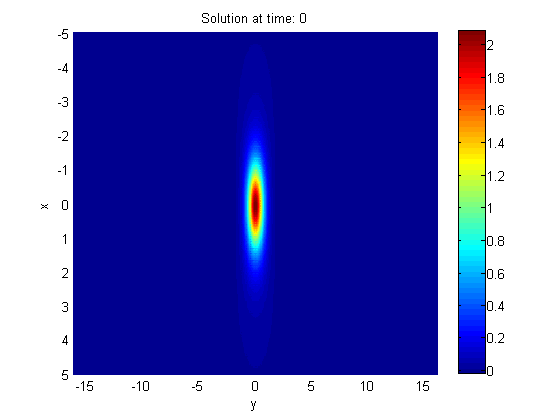
\includegraphics[width=\linewidth]{../amitans/figures/solution_30x45_bt3_c045_T0.png}
	\end{minipage}	
	\begin{minipage}[b]{0.30\linewidth}
		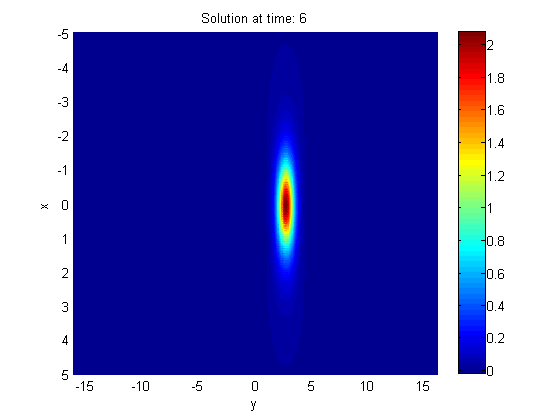
\includegraphics[width=\linewidth]{../amitans/figures/solution_30x45_bt3_c045_T6.png}
	\end{minipage}	
	\begin{minipage}[b]{0.30\linewidth}
		 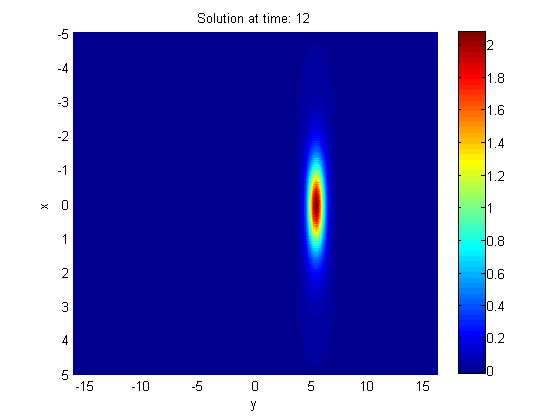
\includegraphics[width=\linewidth]{../amitans/figures/solution_30x45_bt3_c045_T12.png}
	\end{minipage}
	\begin{minipage}[b]{0.30\linewidth}
		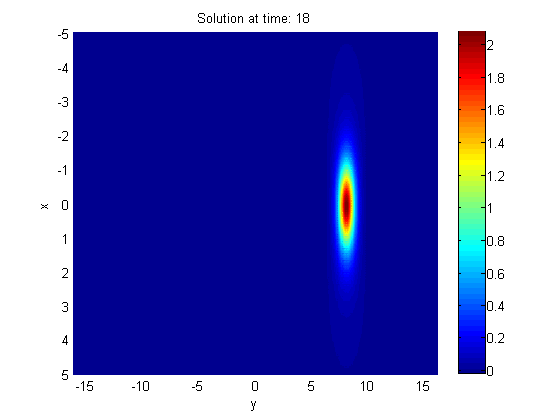
\includegraphics[width=\linewidth]{../amitans/figures/solution_30x45_bt3_c045_T18.png}
	\end{minipage}	
	\begin{minipage}[b]{0.30\linewidth}
		 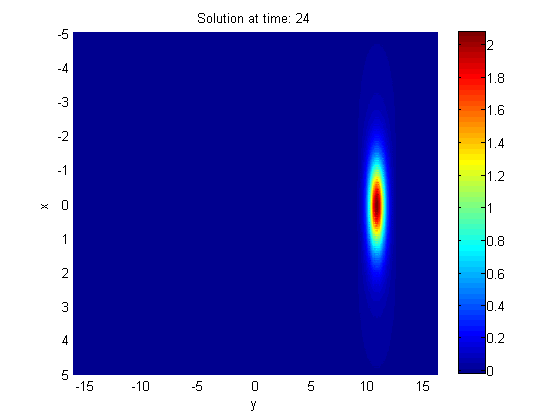
\includegraphics[width=\linewidth]{../amitans/figures/solution_30x45_bt3_c045_T24.png}
	\end{minipage}
	\begin{minipage}[b]{0.30\linewidth}
		 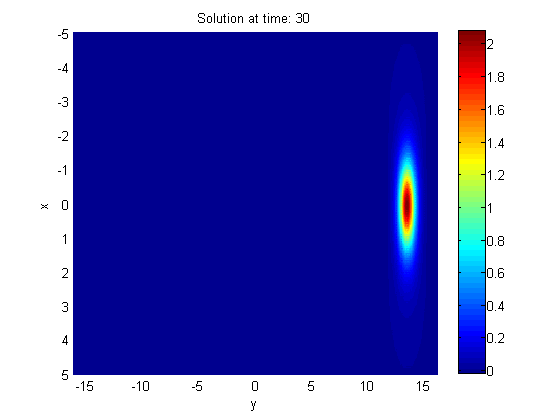
\includegraphics[width=\linewidth]{../amitans/figures/solution_30x45_bt3_c045_T30.png}
	\end{minipage}
\caption{Numerical solution of single wave for $\beta=3$ and $c = 0.45$ at times $t=0,6,12,18,24,30$.}
\label{Wave1}
\end{figure}

\begin{figure}[ht]\vspace{0.2cm}
\centering
	\begin{minipage}[b]{0.30\linewidth}
		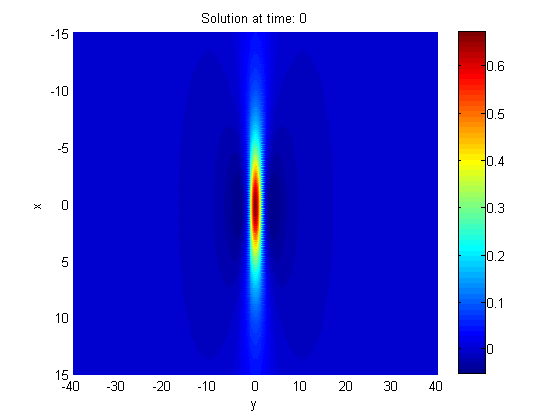
\includegraphics[width=\linewidth]{../amitans/figures/solution_128x90_bt1_c090_T0.png}
	\end{minipage}	
	\begin{minipage}[b]{0.30\linewidth}
		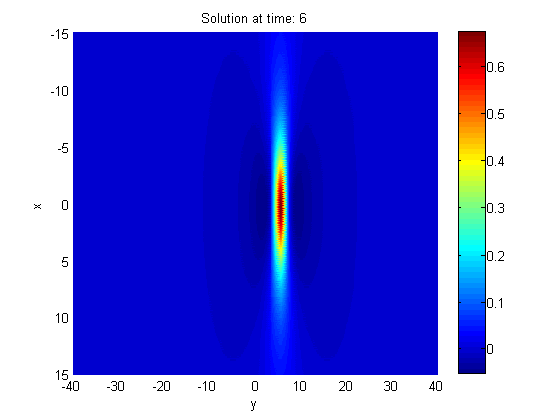
\includegraphics[width=\linewidth]{../amitans/figures/solution_128x90_bt1_c090_T6.png}
	\end{minipage}	
	\begin{minipage}[b]{0.30\linewidth}
		 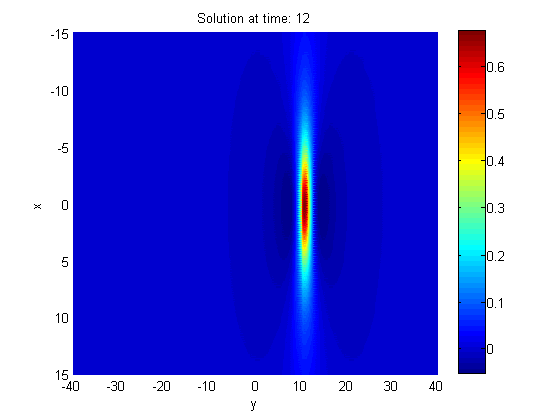
\includegraphics[width=\linewidth]{../amitans/figures/solution_128x90_bt1_c090_T12.png}
	\end{minipage}
	\begin{minipage}[b]{0.30\linewidth}
		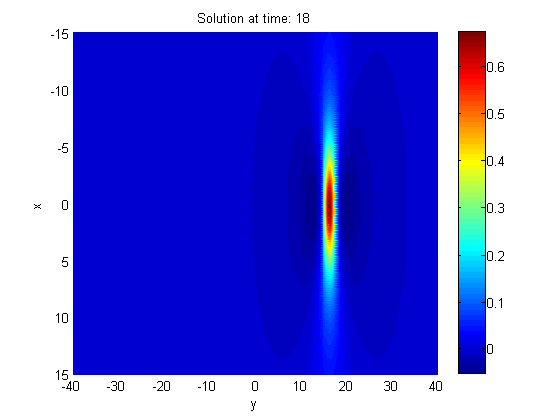
\includegraphics[width=\linewidth]{../amitans/figures/solution_128x90_bt1_c090_T18.png}
	\end{minipage}	
	\begin{minipage}[b]{0.30\linewidth}
		 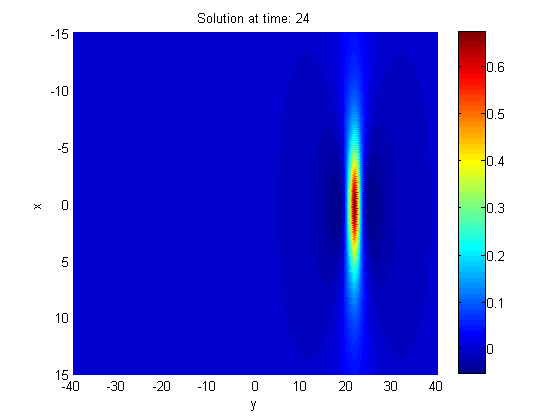
\includegraphics[width=\linewidth]{../amitans/figures/solution_128x90_bt1_c090_T24.png}
	\end{minipage}
	\begin{minipage}[b]{0.30\linewidth}
		 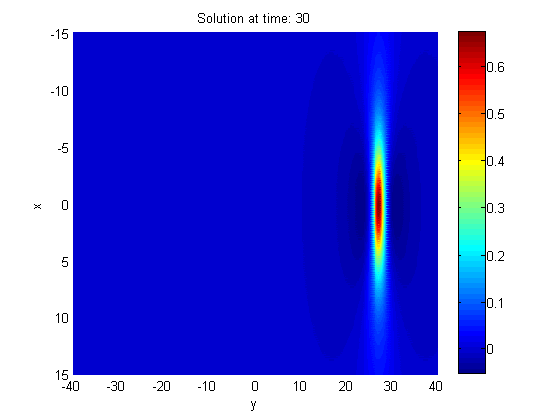
\includegraphics[width=\linewidth]{../amitans/figures/solution_128x90_bt1_c090_T30.png}
	\end{minipage}
\caption{Numerical solution of single wave for $\beta=1$ and $c = 0.9$ at times $t=0,6,12,18,24,30$.}
\label{Wave2}
\end{figure}
The figures are for visual representation. On the contrary, Table \ref{tableF} shows the difference $||uC - uT||_\kappa$ using $L_2$ and infinity norms. The last column of the Table is for the infinity norm of the solution $||uC||_{L_\infty}$ (which is the wave maximum) measured by the Conservative FDS. It is observed that decreasing the step sizes $h$ and $\tau$ results in a smaller difference.  Furthermore the percentage difference when using the infinity norm
$$\frac{ ||uC - uT||_{L_\infty}} { ||uC||_{L_\infty} } \times 100$$
varies in the inteval $[0.0001\%, 0.69\%]$ for all rows in the table. Analogous results are obtained for the percentage difference when using the $L_2$ norm and thus are omitted. The difference between the wave shapes obtained by Conservative FDS and the Taylor Series approach with Method of lines is negligible. It is expected that $||uC - uT||_\kappa$ goes to zero when $h$ and $\tau$ are infinitely small.

%F
\begin{table}[ht]
\centering
\small
		\begin{tabular}{||c|l|l|l|l||}
			\hline
			\hline
      FDS        &$h$, $\tau$  &   $||uC - uT||$  in $L_2$     &  $||uC - uT||$ in $L_\infty$ & $||uC||$ in $L_\infty$ \\
   			\hline 
					\hline 
  $\beta=3$                   &0.2, 0.001         &  1.749e-05      &  1.965e-05  & 1.315448     \\
   c=0.45                        &0.1, 0.0005        &  8.109e-06       & 8.274e-06 &  1.862688     \\
     $O(h^2 + \tau^ 2)$ &0.05, 0.00025     & 2.460e-06         &2.502e-06  &   2.013184   \\
			\hline 
			\hline 
       $\beta=1$          &0.4, 0.002        & 0.009981     & 0.004560 & 0.656747   \\
                  c=0.9      &0.2, 0.001        & 0.005047      & 0.002373  & 0.673901   \\
  $O(h^2+ \tau^2)$ &0.1, 0.0005         & 0.002521      &0.001117 & 0.672231   \\
			\hline
	   \hline
			\hline 
		\end{tabular}
		\caption{Difference $uC - uT$ between solutions from Conservative Scheme and TS approach at time $t=10$ with $O(|h|^2 + \tau^2)$ approximation errors. Differences are measured in $L_2$ and $L_\infty$ norms.}
\label{tableF}
\end{table}

The following paragraph discusses the preservation of the solution's shape over the time interval $[0, 10]$. The set up for the calculations is described in Table \ref{tableP} when using the Taylor method, i.e. $p=2, 4, 6$ and for each approximation order, three nested meshes are used. For more details refer to Table \ref{tableG}. Here, the first column is for the Test case. The second describes the spatial step size $h$. The third and fourth columns present the solution difference at times $t=0$ and $t=10$ in $L_2$ and $L_\infty$ norms. The wave travels a distance which is equal to the speed $c$ multiplied by the end time $T$. Thus, the maximum of the solution at time $t=10$ is located on $(0, 10 c) \in \Omega$. The maximum at time $t=0$ is located on $(0, 0) \in \Omega$. Unfortunately, for Test 1, $h=0.2$ and Test 2, $h=0.4$ the maximum for $t=10$ is not inside the mesh. Further calculations are done to shift the wave along the $y$ axis so that the maximum fall under the closest available meshpoint. For Test 1 ($c=0.45$) the wave travels additional distance of 0.1 for time 2/9 which shifts the maximum to a position of $(0, 4.6) \in \Omega_h$. For Test 2 ($c=0.9$) the wave travels additional distance of 0.2 for time 2/9 which shifts the maximum to a position of $(0, 9.2) \in \Omega_h$. The subtraction of two solutions $u^{(0)} - u^{(N_t)}$ results in a matrix with the following coefficients:
$$ \delta_{i,j} = u_{i,j}^{(0)} - u_{i,j+cT/h}^{(N_t)},$$
where $0 < i < N_x$ and $0 < j < N_y - cT/h$. 

%G
\begin{table}[ht]
\centering
\small
		\begin{tabular}{||c|l|l|l||}
			\hline
			\hline
      FDS        & $h$, $\tau$  & $||u^{(0)} - u^{(N_t)}||$ in $L_2$  & $||u^{(0)} - u^{(N_t)}||$ in $L_\infty$   \\
   		\hline 
			\hline
  $\beta=3$                &0.2, 0.001\footnote{Position of maximum is further adjusted to fit inside $\Omega_h$.}            & 1.494351 & 1.533173    \\
   c=0.45                     &0.1, 0.0005          & 0.466991 & 0.484011       \\
     $O(h^2 + \tau^ 2)$ &0.05, 0.00025   & 0.127641 & 0.132504      \\
			\hline 
  $\beta=3$               &0.2, 0.02 $^{\text{a}}$      &0.220560 & 0.230486       \\
   c=0.45                    &0.1, 0.01      &0.013762 & 0.014391        \\
     $O(h^4+ \tau^4)$ &0.05, 0.005&0.000877 & 0.000917         \\
			\hline 
  $\beta=3$               &0.2, 0.02 $^{\text{a}}$       &  0.035965 & 0.038039        \\
     c=0.45                 &0.1, 0.01        &0.000600 & 0.000633       \\
     $O(h^6+ \tau^6)$ &0.05, 0.005 &0.000010 & 0.000010          \\
	   \hline
			\hline 
       $\beta=1$       &0.4, 0.002 $^{\text{a}}$       & 0.244208 & 0.103833 \\
                  c=0.9    &0.2, 0.001       &  0.057175 & 0.026919  \\
  $O(h^2+ \tau^2)$ &0.1, 0.0005   & 0.013938 & 0.006622  \\
			\hline
      $\beta=1$               &0.4, 0.04 $^{\text{a}}$    &0.028546 & 0.012203 \\
       c=0.9                     &0.2, 0.02     & 0.001757 & 0.000958     \\
       $O(h^4+ \tau^4)$ &0.1, 0.01   & 0.000112 & 0.000061   \\
    \hline
  $\beta=1$                  &0.4, 0.04 $^{\text{a}}$   &0.006415 & 0.002792  \\
      c=0.9                    &0.2, 0.02   &0.000112 & 0.000065     \\
     $O(h^6+ \tau^6)$ &0.1, 0.01 & 0.000002 & 0.000001         \\
	   \hline
			\hline 
		\end{tabular}
		\caption{Difference $||u^{(0)} - u^{(N_t)}||_\kappa$ in $L_2$ and $L_\infty$ norms between solutions at time $t=0$ and $t=10$. TS approach is used for all measurements in the table.}
\label{tableG}
\end{table}

Table \ref{tableG} shows that if the step size $h$ (and $\tau$ respectively) decreases, then the difference also decreases. Furthermore, the shape of the wave is preserved better while the approximation order $p$ increases. Thus, it is expected that $||u^{(0)} - u^{(N_t)}||_\kappa$ goes to zero when $h$ and $\tau$ are infinitely small. 

\begin{figure}\vspace{0.2cm}
	\centering
	\begin{minipage}[b]{0.40\linewidth}
		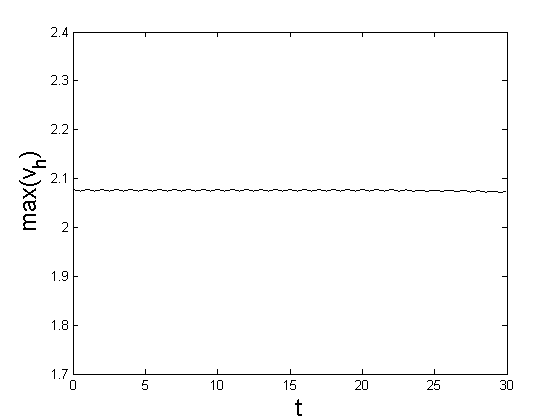
\includegraphics[width=\linewidth]{../amitans/figures/maximum_30_T30_bt3_c045_h005.png}
	\end{minipage}	
	\begin{minipage}[b]{0.40\linewidth}
		 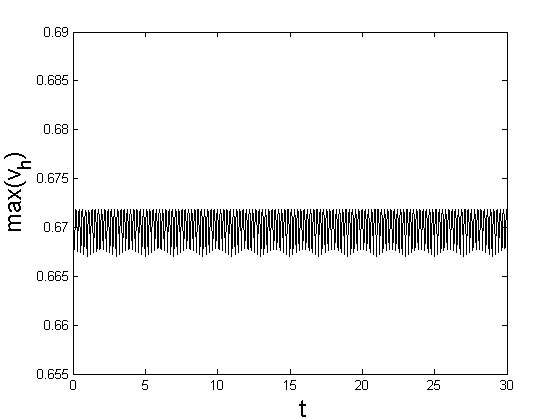
\includegraphics[width=\linewidth]{../amitans/figures/maximum_30_T30_bt1_c090_h020.png}
	\end{minipage}
\caption{Evolution of the maximum over a larger time interval $[0, 30]$ for Test 1 (left panel) and Test 2 (right panel).}
\label{Maximum}
\end{figure}

The following paragraph discusses the maximum of the solution over a larger time interval $[0, 30]$. The set up for the two calculations is described in Table \ref{tableP} where 
$p=6$, $T=30$ and Taylor method is applied with $h=0.05$ and $\tau = 0.001$ for Test 1 and $h=0.2$ and $\tau=0.02$ for Test 2. Also the size of the computational box $\Omega_h$ is extended appropriately along the $y$ axis to compensate for the wave shift. Figure \ref{Maximum} shows that the maximum is stable for both tests over a larger time interval $[0, 30]$. For each iteration step, the exact position of the maximum is not always located on a mesh point in $\Omega_h$. This produces a jagged graph which is well expressed on the right panel and also present on the left panel in Figure \ref{Maximum}. Solution shapes are shown in Figures \ref{Wave1} and \ref{Wave2}.


\begin{thebibliography}{99}

\bibitem{ref16} Angelow, K., Kolkovksa, N., Numercal Study of Traveling Wave Solutions to 2D Boussinesq Equation, {\it Serdica J. Computing}, \textbf{13} (2019), 1-16.

\bibitem{ref0} Boussinesq, J.V., Theorie des ondes et des remous qui se propagent le long d'un canal rectangulaire horizontal, en communiquant au liquide contenu dans ce canal des vitesses sensiblement pareilles de la surface au fond.  {\it Journal de Mathematiques Pures et Appliquees}, \textbf{17} (1872), 55-108.

\bibitem{ref21} Chertok, A., Christov, C.I., Kurganov, A., Central-Upwind Schemes for the Boussinesq Paradigm Equations,
{\it Computational Science and High Performance Computing IV, Notes Numer. Fluid Mech.}, \textbf{113} (2011), 267-281.

\bibitem{ref13}  Christou M. , Christov C.I.,
Galerkin spectral method for the 2D solitary waves of Boussinesq paradigm equation,
In: {\it Applications of Mathematics in Technical and Natural Sciences, Sozopol (Bulgaria)},
\emph{AIP Conference Proceedings}, \textbf{1186}, Issue 1 (2009), 217-225.

\bibitem{ref14}  Christou M. , Christov C.I.,
Fourier Galerkin method for 2D solitons of Boussinesq equation,
{\it Mathematics and Computers in Simulation} \textbf{74} (2007), 82-92.

\bibitem{ref1} Christov, C.I., An energy-consistent dispersive shallow-water model,  {\it Wave Motion}, \textbf{34} (2001), 161-174.

\bibitem{ref15} Christov, C.I., Choudhury, J., Perturbation solution for the 2D Boussinesq equation, {\it Mech. Res. Commun.}, \textbf{38} (2011), 274-281.

\bibitem{ref4} Christov, I., Christov, C.I., Physical dynamics of quasi-particles in nonlinear wave equations,
{\it Physics Letters A}, \textbf{372}, Issue 4 (2008),  841-848.

\bibitem{ref20} Christov, C.I., Kolkovska, N., Vasileva, D., On the Numerical Simulation of Un-
steady Solutions for the 2D Boussinesq Paragigm Equation,
{\it In: I. Dimov, S. Dimova, N. Kolkovska (Eds.), Numerical Methods and Applications 2010},
\emph{Conference Proceedings}, \textbf{6046} (2010), 386–394.

\bibitem{ref23} Dimova M., Vasileva D., Comparison of Two Numerical Approaches to Boussinesq Paradigm Equation, 
{\it Lect. Notes Comput. Sci.}, \textbf{8236} (2013), 255-262.

\bibitem{forn}
Fornberg, B., Generation of Finite Difference Formulas on Arbitrarily Spaced Grids, 
Math. Comput., 51(1988),  699 -- 706.

\bibitem{samarski} Samarskii, A., The Theory of Difference Schemes, Marcel Dekker Inc., New York, 2001.

\bibitem{ref22} Kolkovska, N., Angelow K., A Multicomponent Alternating Direction Method for Numerical Solving of Boussinesq Paradigm Equation,
In: {\it  I. Dimov, I., Farago, I., Vulkov, L. (eds.) NAA 2012},
\emph{Conference Proceedings}, \textbf{8236} (2013), 371–378.

\bibitem{ref25} Kolkovska N., Two families of finite difference schemes for multidimensional Boussinesq paradigm equation, In:
{\it Applications of Mathematics in Technical and Natural Sciences,  Sozopol (Bulgaria)},
\emph{AIP Conference Proceedings}, \textbf{1301} (2010), 395.

\end{thebibliography}
\end{document}